\documentclass{article}\usepackage[]{graphicx}\usepackage[]{color}
% maxwidth is the original width if it is less than linewidth
% otherwise use linewidth (to make sure the graphics do not exceed the margin)
\makeatletter
\def\maxwidth{ %
  \ifdim\Gin@nat@width>\linewidth
    \linewidth
  \else
    \Gin@nat@width
  \fi
}
\makeatother

\definecolor{fgcolor}{rgb}{0.345, 0.345, 0.345}
\newcommand{\hlnum}[1]{\textcolor[rgb]{0.686,0.059,0.569}{#1}}%
\newcommand{\hlstr}[1]{\textcolor[rgb]{0.192,0.494,0.8}{#1}}%
\newcommand{\hlcom}[1]{\textcolor[rgb]{0.678,0.584,0.686}{\textit{#1}}}%
\newcommand{\hlopt}[1]{\textcolor[rgb]{0,0,0}{#1}}%
\newcommand{\hlstd}[1]{\textcolor[rgb]{0.345,0.345,0.345}{#1}}%
\newcommand{\hlkwa}[1]{\textcolor[rgb]{0.161,0.373,0.58}{\textbf{#1}}}%
\newcommand{\hlkwb}[1]{\textcolor[rgb]{0.69,0.353,0.396}{#1}}%
\newcommand{\hlkwc}[1]{\textcolor[rgb]{0.333,0.667,0.333}{#1}}%
\newcommand{\hlkwd}[1]{\textcolor[rgb]{0.737,0.353,0.396}{\textbf{#1}}}%
\let\hlipl\hlkwb

\usepackage{framed}
\makeatletter
\newenvironment{kframe}{%
 \def\at@end@of@kframe{}%
 \ifinner\ifhmode%
  \def\at@end@of@kframe{\end{minipage}}%
  \begin{minipage}{\columnwidth}%
 \fi\fi%
 \def\FrameCommand##1{\hskip\@totalleftmargin \hskip-\fboxsep
 \colorbox{shadecolor}{##1}\hskip-\fboxsep
     % There is no \\@totalrightmargin, so:
     \hskip-\linewidth \hskip-\@totalleftmargin \hskip\columnwidth}%
 \MakeFramed {\advance\hsize-\width
   \@totalleftmargin\z@ \linewidth\hsize
   \@setminipage}}%
 {\par\unskip\endMakeFramed%
 \at@end@of@kframe}
\makeatother

\definecolor{shadecolor}{rgb}{.97, .97, .97}
\definecolor{messagecolor}{rgb}{0, 0, 0}
\definecolor{warningcolor}{rgb}{1, 0, 1}
\definecolor{errorcolor}{rgb}{1, 0, 0}
\newenvironment{knitrout}{}{} % an empty environment to be redefined in TeX

\usepackage{alltt}
\usepackage{Sweave}
\usepackage{float}
\usepackage{graphicx}
\usepackage{tabularx}
\usepackage{siunitx}
\usepackage{amssymb} % for math symbols
\usepackage{amsmath} % for aligning equations
\usepackage{textcomp}
\usepackage{mdframed}
\usepackage[small]{caption}
\setlength{\captionmargin}{30pt}
\setlength{\abovecaptionskip}{0pt}
\setlength{\belowcaptionskip}{10pt}
\topmargin -1.5cm        
\oddsidemargin -0.04cm   
\evensidemargin -0.04cm
\textwidth 16.59cm
\textheight 21.94cm 
%\pagestyle{empty} %comment if want page numbers
\parskip 7.2pt
\renewcommand{\baselinestretch}{2}
\parindent 0pt
\usepackage{lineno}
\linenumbers
\usepackage{natbib}
\bibliographystyle{..//references/styles/besjournalsnew.bst}

%cross referencing:
\usepackage{xr}
\usepackage{xr-hyper}
\externaldocument{/Users/CatherineChamberlain/Documents/git/chillfreeze/docs/chillfrz_supp}

\newmdenv[
  topline=true,
  bottomline=true,
  skipabove=\topsep,
  skipbelow=\topsep
]{siderules}
\IfFileExists{upquote.sty}{\usepackage{upquote}}{}
\begin{document}

\noindent \textbf{\Large{False spring damage to temperate tree saplings is amplified with winter warming}}
%\noindent \textbf{\Large{False springs coupled with warming winters amplify temperate tree damage}}

\noindent Authors:\\
C. J. Chamberlain $^{1,2}$, K. Woodruff $^{1}$ \& E. M. Wolkovich $^{1,2,3}$
\vspace{2ex}\\
\emph{Author affiliations:}\\
$^{1}$Arnold Arboretum of Harvard University, 1300 Centre Street, Boston, Massachusetts, USA 02131; \\
$^{2}$Organismic \& Evolutionary Biology, Harvard University, 26 Oxford Street, Cambridge, Massachusetts, USA 02138; \\
$^{3}$Forest \& Conservation Sciences, Faculty of Forestry, University of British Columbia, 2424 Main Mall, Vancouver, BC V6T 1Z4\\
\vspace{2ex}
$^*$Corresponding author: 248.953.0189; cchamberlain@g.harvard.edu\\

\renewcommand{\thetable}{\arabic{table}}
\renewcommand{\thefigure}{\arabic{figure}}
\renewcommand{\labelitemi}{$-$}
\setkeys{Gin}{width=0.8\textwidth}

%%%%%%%%%%%%%%%%%%%%%%%%%%%%%%%%%%%%%%%%%%%%%%%
%%%%%%%%%%%%%%%%%%%%%%%%%%%%%%%%%%%%%%%%%%%%%%%

\section*{Abstract}
With warming temperatures, spring phenology (i.e., budburst and leafout) is advancing. Late spring freezing events that occur after trees initiate budburst---known as false springs---damage plant tissue and are predicted to increase in certain regions as climate change progresses. Additionally, over-winter chilling temperatures may decrease as winter temperatures warm, potentially impacting phenology and, ultimately, growth. If over-winter chilling is too low in a season, plants may leaf out much slower or incompletely, subsequently decreasing spring freeze tolerance. Understanding the intersection of warming winters and false spring risk is critical to predict how temperate forests will change in the future. Here, we assessed the effects of varying durations of over-winter chilling on sapling phenology and growth across eight temperate tree and shrub species. Half of the individuals were then exposed to false spring conditions. We found that false springs increased the rate of budburst, increased damage to the shoot apical meristem, and decreased leaf toughness, leaf thickness and chlorophyll content but did not cause phenological reordering within a community. Longer chilling led to decreased rates of budburst, even under false spring conditions, thus chilling compensated for the adverse effects of false springs on phenology. We therefore expect climate change to reshape forest communities not through temporal reassembly but rather through impacts on growth and leaf traits from the coupled effects of false springs with decreases in over-winter chilling under future climate change scenarios.

\textbf{Synthesis:} With climate change and warming temperatures, over-winter chilling is anticipated to decrease and false springs are predicted to increase in certain regions. This combination could greatly impact plant performance, survival and shape species distributions, ultimately affecting crucial processes such as carbon uptake and nutrient cycling.

\vspace{2ex}
\textit{Keywords:} false spring, climate change, phenology, spring freeze, forest recruitment, temporal reassembly, budburst, temperate

\section*{Introduction}
%EMWAug14 -- first two paragraphs are good, but I think could be a little tighter -- ask a colleague or two to review and see what they think? Could just be me ....
The timing of spring in temperate deciduous forests shapes plant and animal communities and influences ecosystem services from agriculture to forest management. With warming temperatures, spring phenology (i.e., budburst and leafout, which are strongly cued by temperature) is advancing, causing longer growing seasons \citep{Chuine2001} and reshaping these services. In one major example, advancing spring phenology has led to increased carbon uptake across temperate forests, which are essential carbon sinks that combat the negative effects of climate change \citep{Keenan2014}. But climate change could diminish or reverse these positive effects on carbon storage: specifically through cold snaps during the spring and reduced cool temperatures in the winter.
  
While climate change has warmed the Northern Hemisphere, extreme weather events (e.g., polar vortexes) are still occurring. These weather events can have big impacts on plant development each spring. One such event is known as a `false spring', which is when temperatures drop below freezing \citep[][i.e., below -2.2$^{\circ}$C]{Schwartz2002} after budburst has initiated. Damage from false spring events can have cascading effects to pollinators \citep{Boggs2012, Pardee2017}, nutrient cycling and carbon uptake as well as forest recruitment \citep{Hufkens2012, Klosterman2018, Richardson2013}.

Furthermore, false springs can increase the chance of additional freezes within a growing season by extending the period in which plants are most at risk---the time between budburst and leafout (what we refer to as the `duration of vegetative risk'). Observational studies suggest plants take longer to re-flush leaves after a false spring---up to 38 days \citep{Augspurger2009, Augspurger2013, Gu2008, Menzel2015}, which could lead to additional false springs in a season \citep{Augspurger2009}. False springs are predicted to increase in certain regions as climate change progresses \citep{Ault2015, Liu2018, Zohner2020}, thus understanding the impacts of false spring events on forests is essential for forest management strategies and climate forecasting \citep{OBrien2019}. 
  
Warmer winters may also play a critical role in the future of forests as they directly impact one of the  major cues plants use to time budburst: over-winter cold temperatures (chilling), in addition to warming spring temperatures (forcing) and longer daylengths. Many temperate plants have evolved chilling requirements to avoid leafout during warm snaps in the middle of the winter, but with climate change, chilling requirements may not be met. If chilling is not met, plants may leaf out much slower or incompletely, which can in turn affect freeze tolerance. Thus, understanding the interplay of warming winters and false spring risk is critical to predict how temperate forests will change in the future.
  
This interaction between winter chilling and false springs may vary across species within a community. This is especially true if species have evolved along a trade-off of risking spring freezes for early access to resources: while ideally all individuals of all species would evolve to require high levels of chilling to delay budburst and ultimately diminish false spring risk but competition for nutrients, water and light resources in the early spring likely pushes individuals to leafout earlier \citep{Augspurger2013}. Young trees and understory species generally initiate budburst before the canopy trees to benefit from higher light levels \citep {Augspurger2008, Vitasse2013}, which potentially puts these species and individuals at higher risk of freeze damage \citep{Vitasse2014}. Thus, successful forest recruitment requires seedlings and saplings to minimize false spring risk while maximizing growth. 
 
The combination of species- and lifestage-level differences in responses to false springs, chilling and climate change could reshape the temporal assembly of forest communities. Species typically leafout in a similar sequence, with understory species leafing out earlier and higher canopy trees leafing out last but many studies are predicting substantial shifts in chronological order and reassembly of species' leafout with climate change \citep{Roberts2015, Laube2014}. As warming alters winter temperatures and false spring prevalence, phenological cues and their interactions are anticipated to change, which could greatly alter competition and recruitment among forest species for early season resources and ultimately impact species diversity and carbon uptake in temperate forests.
  
Here, we assessed the effects of over-winter chilling length and false springs on sapling phenology and growth across eight temperate tree and shrub species. We exposed individuals to different levels of over-winter chilling crossed with a false spring event in growth chambers, following individuals for a growing season to ask: (1) How does over-winter chilling (2) how do false spring events impact phenology, growth and physical leaf traits and (3) how does the interaction between chilling and false springs impact community structure and phenological order?

\section*{Materials and Methods} %EMW12Aug: Lots of edits throughout, mostly to switch to active voice where easy and to make it shorter. A few places you repeated things so I deleted those spots -- let me know if I accidentally deleted anything important!
\subsection*{Plant Selection and Material}
We selected eight temperate woody plant tree and shrub species that span varying spring phenologies (e.g., early to later leafout), that were not used as crops or ornamental species: \textit{Acer saccharinum} L., \textit{Alnus incana rugosa} L., \textit{Betula papyrifera} Marsh., \textit{Betula populifolia} Marsh., \textit{Cornus racemosa} Lam., \textit{Salix purpurea} L., \textit{Sorbus americana} Marsh., and \textit{Viburnum dentatum} L. (we originally included two additional species---\textit{Fagus grandifolia} and \textit{Nyssa sylvatica}, but the plants were not delivered in a usable condition and thus we excluded them from the experiment). We used 48 dormant, one year old, bare root saplings---each measuring 6-12 inches---for each species from Cold Stream Farm LLC (Freesoil, MI; 44$^{\circ}$6' N -86$^{\circ}$12' W) for a total of 384 individuals. Upon receipt, plants were potted in 656ml deepots with Fafard \#3B Metro Mix soil and placed in growth chambers at the Weld Hill Research Building of the Arnold Arboretum (Boston, MA; 42$^{\circ}$17' N -71$^{\circ}$8' W) at 4$^{\circ}$C for different durations depending on chilling conditions.  %EMW12Aug: Are you required to use the L. for the journal? I would skip it otherwise; better to reference a current flora that shows all these species that 'L.' 

\subsection*{Growth Chamber and Greenhouse Conditions}
Individuals were randomly selected for one of six experimental treatments from a full factorial design of false spring (two levels: presence or absence of false spring) x chilling (three levels: four, six or eight weeks of chilling at 4$^{\circ}$C with eight hour photoperiod, lighting was a combination of T5HO fluorescent lamps with halogen incandescent bulbs at roughly 250 $\mu mol/m^{2}/s$). Individuals were rotated within and among growth chambers every two weeks to eliminate bias from possible growth chamber effects.

Once chilling was completed, we moved individuals to a greenhouse with mean daytime temperature of 15$^{\circ}$C and a mean nighttime temperature of 10$^{\circ}$C, and a photoperiod of 12 hour days throughout the spring until all individuals reached full leaf expansion. After all individuals of all species reached full leaf expansion, greenhouse temperatures and photoperiods were kept ambient, and all individuals were up-potted to 983ml deepots and fertilized with SCOTTS 15-9-12 Osmocote Plus 5-6. 

\subsection*{Phenology and False Spring Treatment}
We recorded phenology (using the BBCH scale) every 2-3 days through full leaf expansion. Budburst was denoted as BBCH stage 07, which is `beginning of sprouting or bud breaking' and monitored until full leaf expansion (BBCH stage 19) in order to evaluate the duration of vegetative risk \citep{Chamberlain2019} for each individual \citep{Finn2007}. Individuals in the `false spring treatment' were placed in a growth chamber set to mimic a false spring event during budburst, defined as once at least 50\% of the buds were at BBCH stage 07 but the individual had not yet reached BBCH stage 19 (that is, each individual was exposed to a false spring based on its individual phenological timing). False spring treatments lasted approximately 14 hours, beginning at 6pm; temperatures were ramped down over 14 hours (Figure \ref{fig:gccond}). Around 8am the following day, we placed false spring individuals back in the greenhouse. Once all individuals reached full leaf expansion (BBCH stage 19), we recorded phenology weekly until August 1st, then every 2-3 days again to monitor fall phenology. We monitored all individuals until complete budset. 

\subsection*{Growth measurements}
We measured height three times throughout the growing season (the day an individual reached full leaf expansion, 60 days after full leaf out and when an individual reached complete budset). We measured the chlorophyll content of four leaves on each individual 60 days after full leaf out using an atLEAF CHL PLUS Chlorophyll meter, converting chlorophyll content to mg/cm\textsuperscript{2} using the atLEAF CHL PLUS conversion tool. We measured leaf thickness using a Shars Digital Micrometer (accurate to 0.001mm) and leaf toughness in Newtons using a Shimpo Digital Force Gauge on two leaves for each individual 60 days after full leaf out. Additionally, we visually monitored damage to the shoot apical meristem, which consisted of complete damage or disruption of growth in the main stem and resulted in early dormancy induction or reliance on lateral shoot growth. Finally, we harvested each plant after it reached complete budset to dry, separate and weigh belowground and aboveground biomass (including leaves). 

\subsection*{Data analysis}
We used Bayesian hierarchical models (with the brms package \citep{brms}, version 2.3.1,  in R \citep{R}, version 3.3.1) to estimate the effects of chilling duration, false spring treatment and all two-way interactions as predictors on: (1) duration of vegetative risk, (2) growing season length, (3) shoot apical meristem damage, (4) total growth in centimeters, (5) total biomass, (6) chlorophyll content, (7) leaf toughness and (8) leaf thickness. We modeled species hierarchically as grouping factors, which generated an estimate and posterior distribution for each species as well as an overall response across the eight species used in our experiment. We ran four chains, each with 4 000 iterations, of which 2 500 were warm-up iterations, for a total of 6 000 posterior samples for each predictor for each model using weakly informative priors (increasing priors three-fold did not impact our results). We evaluated our model performance based on $\hat{R}$ values that were close to one, checked chain convergence and posterior predictive checks visually \citep{BDA}, and made sure all models had 0 divergent transitions. Our models generally had high $n_{eff}$ (4000 for most parameters, but as low as 1400 for a couple of parameters in the shoot apical meristem model). All estimated values are reported in the text as means +/- standard errors relative to the no false spring under four weeks of chilling treatment.


\section*{Results} 
Chilling durations impacted individual phenology. As seen in many other studies, we found increases in chilling advanced day of budburst by -2.8 $\pm$ 1.7 days for six weeks of chilling and by -7.6 $\pm$ 1.8 days for eight weeks of chilling (as mentioned above, all values are given relative to the no false spring under four weeks of chilling treatment; Table \ref{tab:simpbb}). Longer chilling also sped up leafout, reducing the duration of vegetative risk (8 weeks: -2.7 $\pm$ 1.1 days; Figure \ref{fig:muphen}\textbf{a}, Table \ref{tab:simpdvr} and Table \ref{tab:suppmoddvr}). Increased chilling shortened the growing season for individuals exposed to six and eight weeks of chilling (6 weeks: 2.5 $\pm$ 4.9 days; 8 weeks: -9.7 $\pm$ 5 days; Figure \ref{fig:muphen}\textbf{b} and Table \ref{tab:suppmodgs}). Individuals under six and eight weeks of chilling were put in the greenhouse two to four weeks later than the four weeks of chilling group but all individuals experienced the same ambient conditions when in the greenhouse. Due to experimental design constraints, growing season length was shortened for the groups that experienced longer chilling.
 
False springs also impacted individual phenology. Individuals exposed to the false spring treatment had longer durations of vegetative risk given four weeks of chilling (3 $\pm$ 0.8 days) and slightly longer durations for given six weeks of chilling (1.6 $\pm$ 1.1 days; Figure \ref{fig:muphen}\textbf{a} and Table \ref{tab:suppmoddvr}). Effects on the duration of vegetative risk from false spring treatments (which led to longer durations) and from increased chilling (which led to shorter durations) were generally additive, resulting in no major changes in the durations of vegetative risk for individuals exposed to a false spring that received eight weeks of chilling (0.9 $\pm$ 1.1 days, Figure \ref{fig:muphen}\textbf{a} and Table \ref{tab:suppmoddvr}). 

False springs impacted growth habit and shoot growth but not total biomass. Across all chilling treatments, especially for the four and eight week chilling treatments, false springs led to more damage to the shoot apical meristem (4 weeks: 52.5\% increase in probability of damage under false spring treatment or 2.1 $\pm$ 1; 6 weeks: 35\% or a 1.4 $\pm$ 1.4; and 8 weeks: 55\% or a 2.2 $\pm$ 1.3; Figure \ref{fig:mugrowth}\textbf{a} and Table \ref{tab:suppmodmeri}). Shoot growth over the growing season increased with eight weeks of chilling (11 $\pm$ 4 cm) but growth did not increase for eight weeks of chilling under false spring conditions (4.8 $\pm$ 5.5 cm; Figure \ref{fig:mugrowth}\textbf{b} and Table \ref{tab:suppmodht}). False springs led to slightly lower total biomasses when they were exposed to only four weeks of chilling (-3.4 $\pm$ 2.8 g) but there was very little change in total biomass under false spring conditions (compared to the no false spring) for both the six (-3.5 $\pm$ 4 g) and the eight weeks of chilling treatments (2.9 $\pm$ 3 g; Figure \ref{fig:mutotbio} and Table \ref{tab:suppmodtotbio}).
  
False springs also affected physical leaf traits. False spring treatments decreased leaf toughness across all chilling treatments (4 weeks: -0.1 $\pm$ 0 N; 6 weeks: -0.2 $\pm$ 0 N; and 8 weeks: -0.2 $\pm$ 0 N; Figure \ref{fig:muleaf}\textbf{a} and Table \ref{tab:suppmodtough}) and decreased chlorophyll content in leaves with six and eight weeks of chilling (6 weeks: -1.5 $\pm$ 1.2 mg/cm\textsuperscript{2}; and especially for 8 weeks: -2.1 $\pm$ 1.1 mg/cm\textsuperscript{2}; Figure \ref{fig:muchl} and Table \ref{tab:suppmodchl}). Additionally, false springs led to decreased leaf thickness across four and eight weeks of chilling treatments, but there was little change for the six weeks of chilling treatment (4 weeks: -8.9 $\pm$ 3.7 $\mu$m; 6 weeks: -3.5 $\pm$ 5.3 $\mu$m; and 8 weeks: -15.8 $\pm$ 5.3 $\mu$m for eight weeks of chilling; Figure \ref{fig:muleaf}\textbf{b} and Table \ref{tab:suppmodthick}). 
  
False springs and chilling treatments were generally consistent across species, though not always. Duration of vegetative risk decreased for most species with longer chilling (i.e., the eight weeks), except for \textit{Salix purpurea}, which experienced longer durations of vegetative risk with longer chilling (Figure \ref{fig:muphen}\textbf{a}). False springs led to meristem damage agross all species except for \textit{Betula populifolia} and \textit{Sorbus americana}. Additionally, \textit{Viburnum dentatum} experienced consistent meristem damage under all treatments (Figure \ref{fig:mugrowth}\textbf{a}). Effects on leaf thickness were especially variable across species under the longer chilling treatments, specifically with \textit{Sorbus americana} and \textit{Viburnum dentatum} having thicker leaves with increased chilling (Figure \ref{fig:muleaf}\textbf{b}). 
  
Despite large treatment effects on phenology, we found no major effects on phenological rank within the community. Order of leafout timing was consistent across all treatments, with \textit{Salix purpurea} always being first to leafout, followed by \textit{Betula papyrifera}, \textit{B. populifolia} and \textit{Cornus racemosa}, followed by \textit{Alnus rugosa}, \textit{Sorbus americana}, \textit{Viburnum dentatum} and \textit{Acer saccharinum} (Figure \ref{fig:rank}). \textit{Viburnum dentatum} was the only species to change rank across treatments, though it was consistently grouped with the later-leafout  species. Order of budset timing was also consistent across all treatments, with \textit{Cornus racemosa} and \textit{Sorbus americana} being first to set bud, followed by \textit{Betula papyrifera}, \textit{Acer saccharinum} and \textit{Viburnum dentatum}, followed by \textit{B. populifolia}, \textit{Salix purpurea} and \textit{Alnus rugosa} (Figure \ref{fig:bsetrank}). \textit{Acer saccharinum} was the only species to change budset rank across treatments, though it was grouped consistently with \textit{Betula papyrifera} and \textit{Viburnum dentatum}.

\section*{Discussion} 
Our experiment allowed us to examine the consequences of two major interactive effects of climate change across eight deciduous forest tree species---false springs and chilling. Our results confirmed the major features of false springs (plant damage) and chilling (advancing spring phenology) then highlighted how these two effects altered multiple aspects of plant phenology, plant growth and leaf traits. Importantly, we found false springs and chilling have opposing additive effects on the duration of vegetative risk. This suggests that the combination of increased false springs and warmer winters could be especially detrimental to forest communities.

\subsection*{False springs and chilling interactively determine risk and damage}
Chilling length greatly influences spring phenology during the critical budburst to leafout phases, and thus may compensate for the detrimental effects of false springs on phenology. With false springs increasing the duration of vegetative risk, the risk of multiple false springs occurring in one season also increases. But our experiment found that chilling can compensate for this increase in duration of vegetative risk: with increased chilling, the duration of vegetative risk does not increase under false spring conditions. This suggests chilling is more important for saplings in terms of exposure to multiple false springs. With climate change and warming temperatures, over-winter chilling is anticipated to decrease \citep{Laube2014} and false springs are predicted to increase in certain regions \citep{Ault2015, Liu2018}. This combination could greatly impact plant performance, survival and shape species distributions, ultimately affecting ecosystem processes, such as carbon uptake and nutrient cycling.
 
We found that false springs impacted sapling growth, regardless of chilling duration. Past studies suggest early-budburst species can withstand lower temperature thresholds \citep{Lenz2013, Muffler2016, Zohner2020} but our results suggest false springs consistently impair shoot apical meristem growth, regardless of a species phenological order. Damage to the shoot apical meristem can lead to reliance on lateral shoot growth, rendering inefficient growth patterns and---if damage is significant within a forest stand---it can lead to declines in recruitment \citep{Rhodes2018}. Though overall height increased with more over-winter chilling, false springs impacted all individuals similarly across all chilling treatments, suggesting an interplay between false spring damage to the meristem and overall plant height and thus further emphasizing the detrimental effects of meristem damage.   
  
False springs greatly impacted the physical characteristics of the leaf in our experiment: with chlorophyll content, leaf toughness and leaf thickness decreasing, the quality of the leaf decreased. This reduction in quality could subsequently lead to an increase in herbivory risk \citep{Onoda2011}. We found that increased chilling levels decreased leaf toughness and decreased chlorophyll content under false spring conditions. Further studies that assess the secondary compounds and total phenolic content \citep{Ayres1993, Webber2016} as well as photosynthetic rate of the leaves are needed to better assess the interactive effects of chilling and false springs on leaf level traits and better predict herbivory risk and the overall leaf quality under climate change. 

\subsection*{False springs and chilling do not reshape temporal assembly}
Climate model projections and experimental studies with very low chilling predict substantial shifts in species leafout order under future climate change conditions \citep{Roberts2015, Laube2014}; other studies using long-term phenology observations suggest leafout phenology order is consistent across years \citep{Wesolowski2006}. We did not find major shifts in species leafout order---thus consistent with observational studies \citep{Wesolowski2006}---except for \textit{Viburnum dentatum}, though it still leafed out within the late-leafout group of species across all treatments. Therefore, we do not predict major reassembly of forest communities due to winter warming or false spring incidence. Our results are also in line with some experimental studies, for example, in one full factorial growth chamber experiment, most treatments did not lead to substantial phenological reordering, except when individuals experienced little to no field chilling \citep{Laube2014}. Future climate projections suggest major shifts in chilling due to warmer winters, which our design may not fully capture, but chilling is also not well understood \citep{Nanninga2017}. Some regions may experience more chilling rather than less with warming (CITE - check budburst paper). Given that we found chilling has cascading effects on phenology, growth and leaf traits, we need to better understand over-winter chilling in order to make accurate predictions. 
    
Phenological rank remained consistent across all our false spring and chilling treatments---where all species were affected equally. In nature, not all of our study species are at equal risk of false springs, with early-budburst species (e.g., \textit{Salix americana} or \textit{Betula papyrifera}) generally more at risk than later-budburst species (e.g., \textit{Acer saccharinum} or \textit{Viburnum dentatum}). This suggests that climate change could reshape forest communities, though not directly through temporal assembly. Instead, our results suggest that change may come from physical damage and leaf trait impacts of false springs and decreases in chilling. Some temperate tree and shrub species utilize various leaf characteristics to lower their risk of false spring damage: increased `packability' of leaf primordia in winter buds, which allows for more rapid leafout \citep{Edwards2017}, increased trichome density on young leaves to protect leaf tissue against freezes \citep{Agrawal2004, Prozherina2003} and buds with decreased water content to increase freeze tolerance \citep{Beck2007, Hofmann2015, Kathke2011, Morin2007,  Muffler2016, Nielsen2009, Poirier2010}. Thus, it is crucial to better understand how these freeze tolerance physiologies differ among species and if they are anticipated to change with warming but ultimately we found that the complex interplay of a changing climate and species-specific mosaics of traits could influence phenological rank and forest community structure. 

Our results suggest that predicting future forest recruitment will require integrating the effects of shifting false springs on inter- and intraspecific competition. With over-winter chilling decreasing with climate change, saplings---which generally leafout earlier than later lifestages to gain access to light \citep{Augspurger2009}---are likely more at risk of damage from false spring events. This could lead to dieback of saplings, most especially of early-budbursting species, in temperate forests with climate change. Thus, climate change could greatly impact early-budburst species, which will likely see increases in durations of vegetative risk from the dual effects of lower chilling and heightened false spring risk. Understanding how false springs are changing and how equally---or not---these effects are on different species and their seedlings is crucial for future projections. By integrating the additive and adverse effects of decreasing over-winter chilling and increasing false spring risk---and how false springs are changing across various species, we can better predict shifts in forest communities and recruitment under climate change. 

\section*{Acknowledgments}
We would like to thank all of the growth facilities staff at the Weld Hill Research Building with a special thanks to K. Woodruff, F. Rosin and W. Daly for their continued dedication to the project and greenhouse and laboratory assistance. We also thank D. Buonaiuto, A. Ettinger, J. Gersony, D. Loughnan, A. Manandhar and D. Sohdi for their continued feedback and insights that helped improved the experimental design, questions and manuscript.

\section*{Author Contribution} 
C.J.C. and E.M.W. conceived of the study and analysis and identified species to use in the study and determined which phenological and growth measurements to observe. C.J.C. performed the analyses and produced all figures and tables. C.J.C. wrote the paper, and both authors edited it.

\section*{Data Availability:}
Data and code from the analyses will be available via KNB upon publication and are available to all reviewers upon request. Raw data, {Stan} model code and output are available on github at \url{https://github.com/cchambe12/chillfreeze} and provided upon request.


\bibliography{..//references/chillfreeze.bib}

\section*{Tables and Figures}

{\begin{figure} [H]
  -\begin{center}
  -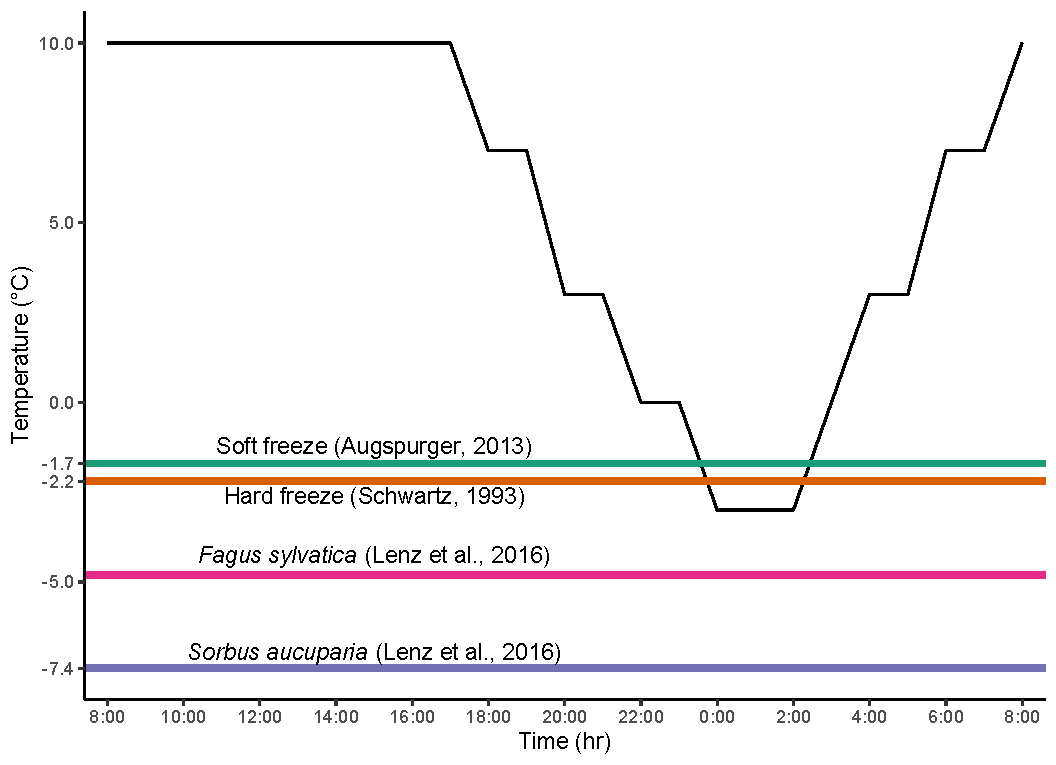
\includegraphics[width=12cm]{..//analyses/figures/growthchamber.pdf}
  -\caption{False spring treatment temperature regime in the growth chamber}\label{fig:gccond}
  -\end{center}
  -\end{figure}}
  
  {\begin{figure} [H]
  -\begin{center}
  -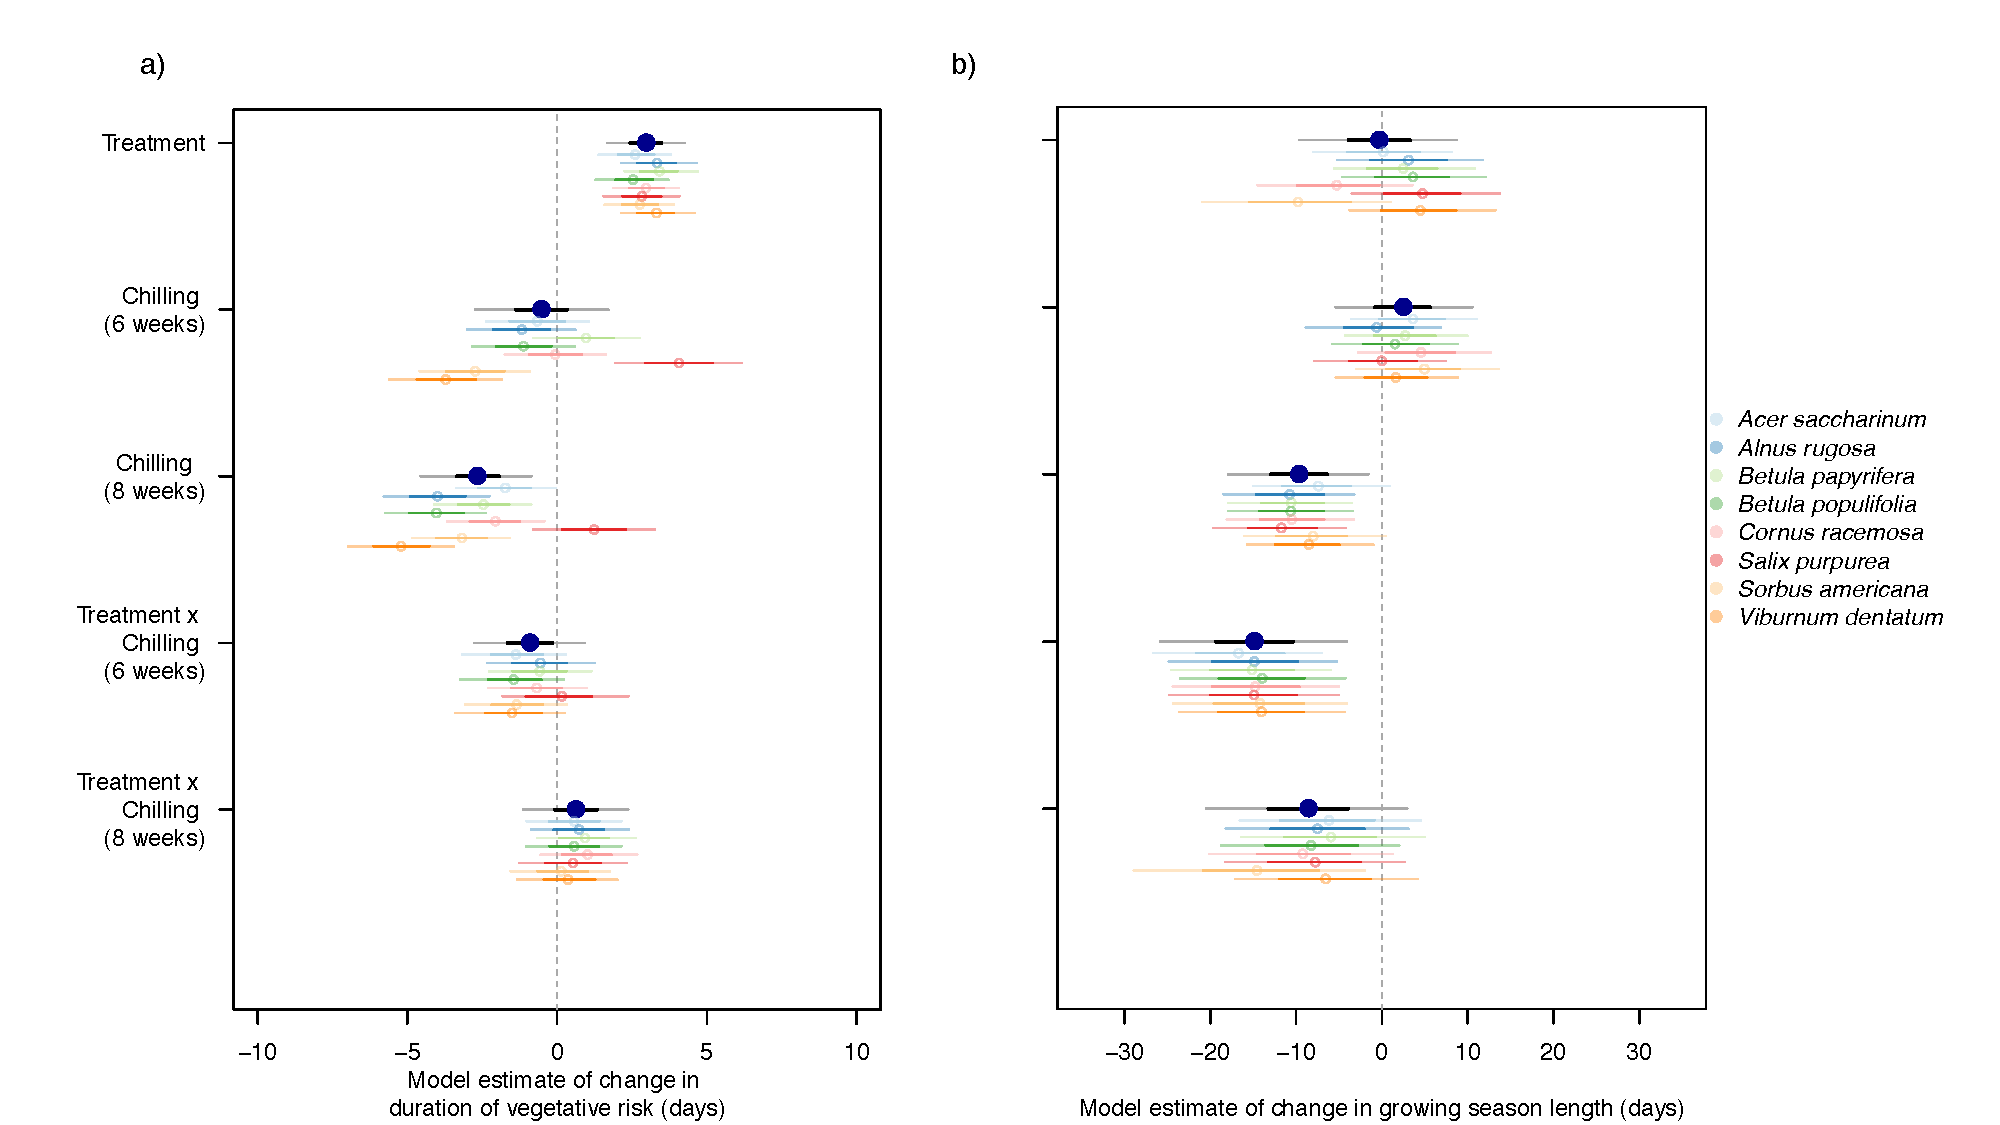
\includegraphics[width=18cm]{..//analyses/figures/mu_phen.pdf} 
  -\caption{Effects of false spring treatment, six weeks of chilling and eight weeks of chilling on a) duration of vegetative risk (days) and b) growing season length (days). Dots and thin lines show means and 90\% uncertainty intervals and thicker lines show 50\% uncertainty intervals.}\label{fig:muphen} %EMWAug14 -- for first figure add the baseline (4 weeks chill x no false spring) that they're all relative to?
  -\end{center}
  -\end{figure}}
  
  {\begin{figure} [H]
  -\begin{center}
  -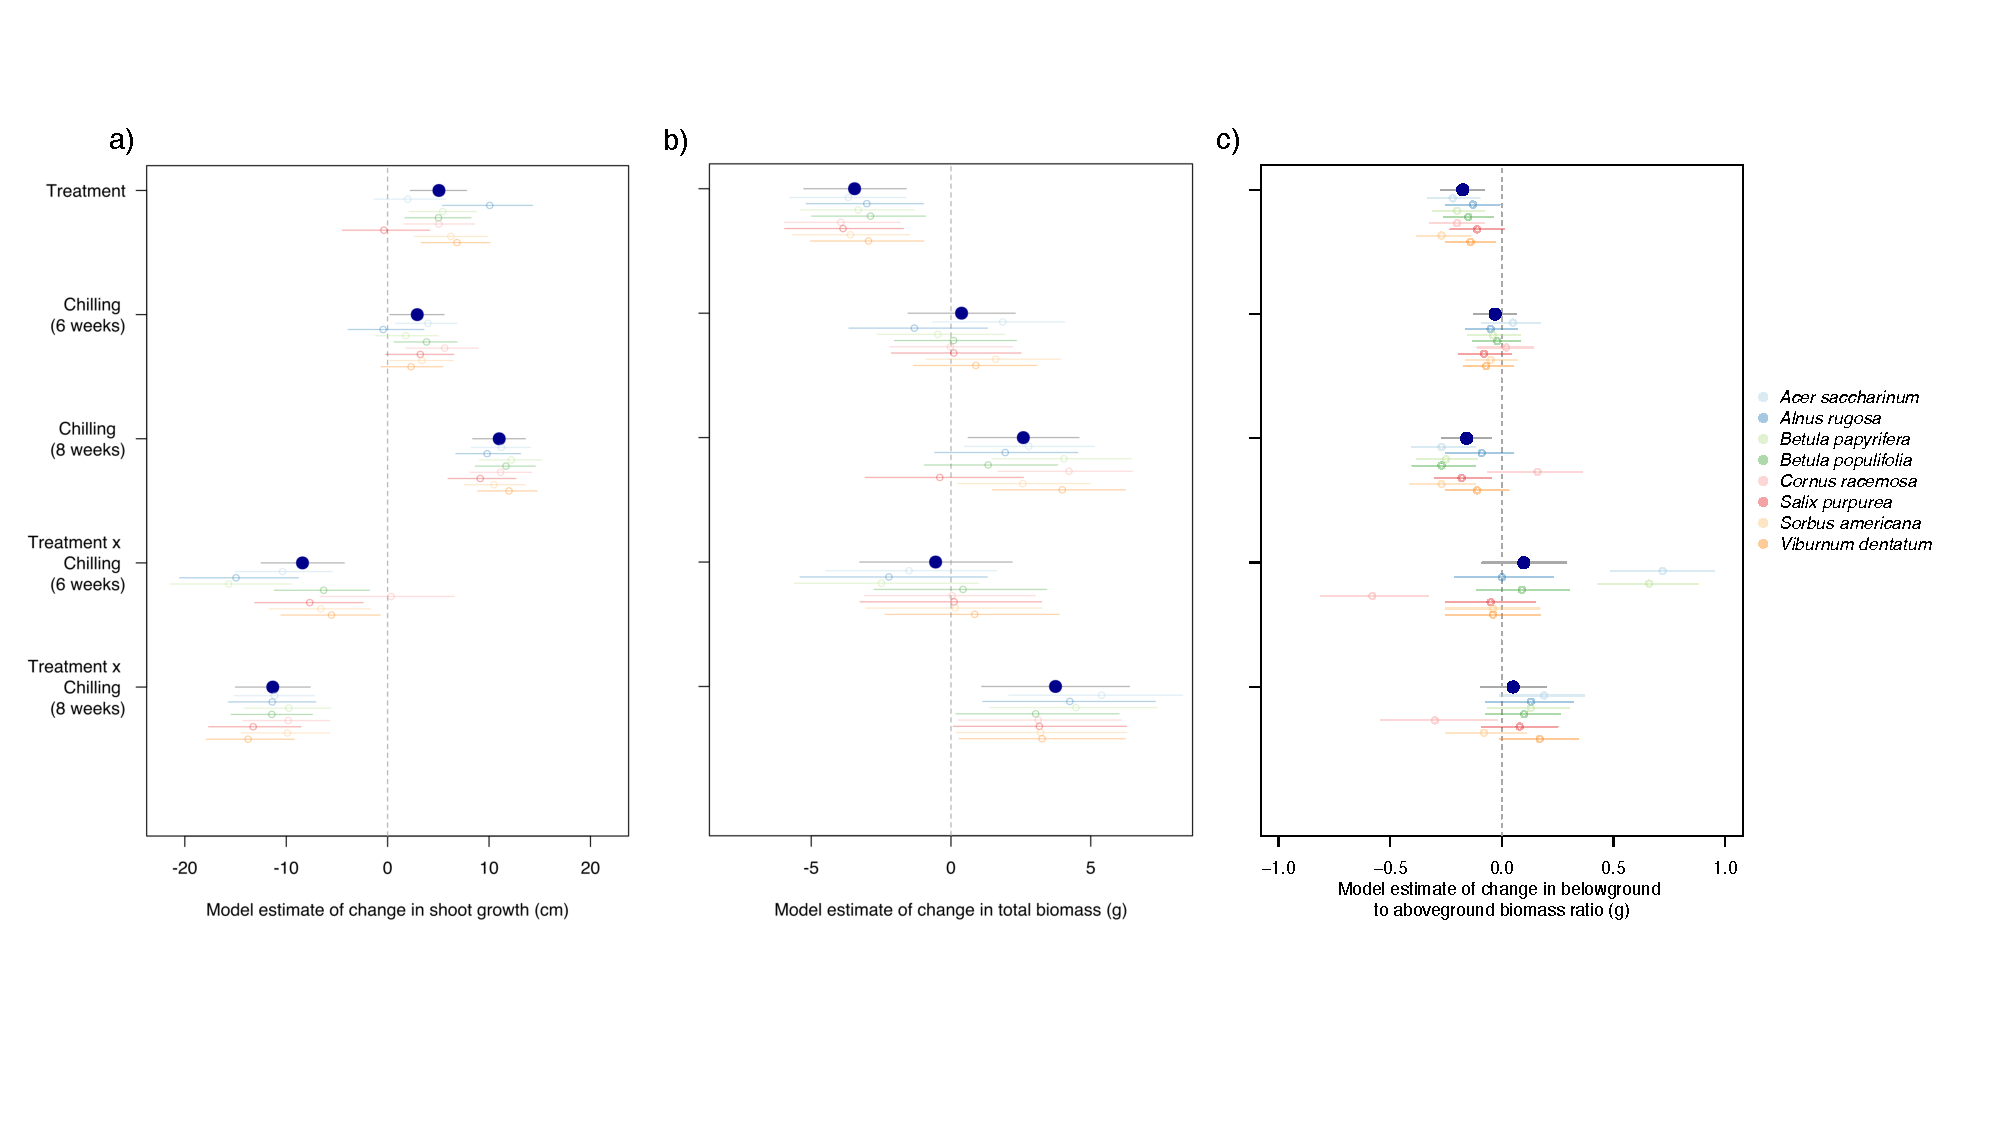
\includegraphics[width=18cm]{..//analyses/figures/mu_growth.pdf} 
  -\caption{Effects of false spring treatment, six weeks of chilling and eight weeks of chilling on a) shoot apical meristem damage and b) total shoot growth (cm). Dots and thin lines show means and 90\% uncertainty intervals and thicker lines show 50\% uncertainty intervals. }\label{fig:mugrowth}
  -\end{center}
  -\end{figure}}
  
  {\begin{figure} [H]
  -\begin{center}
  -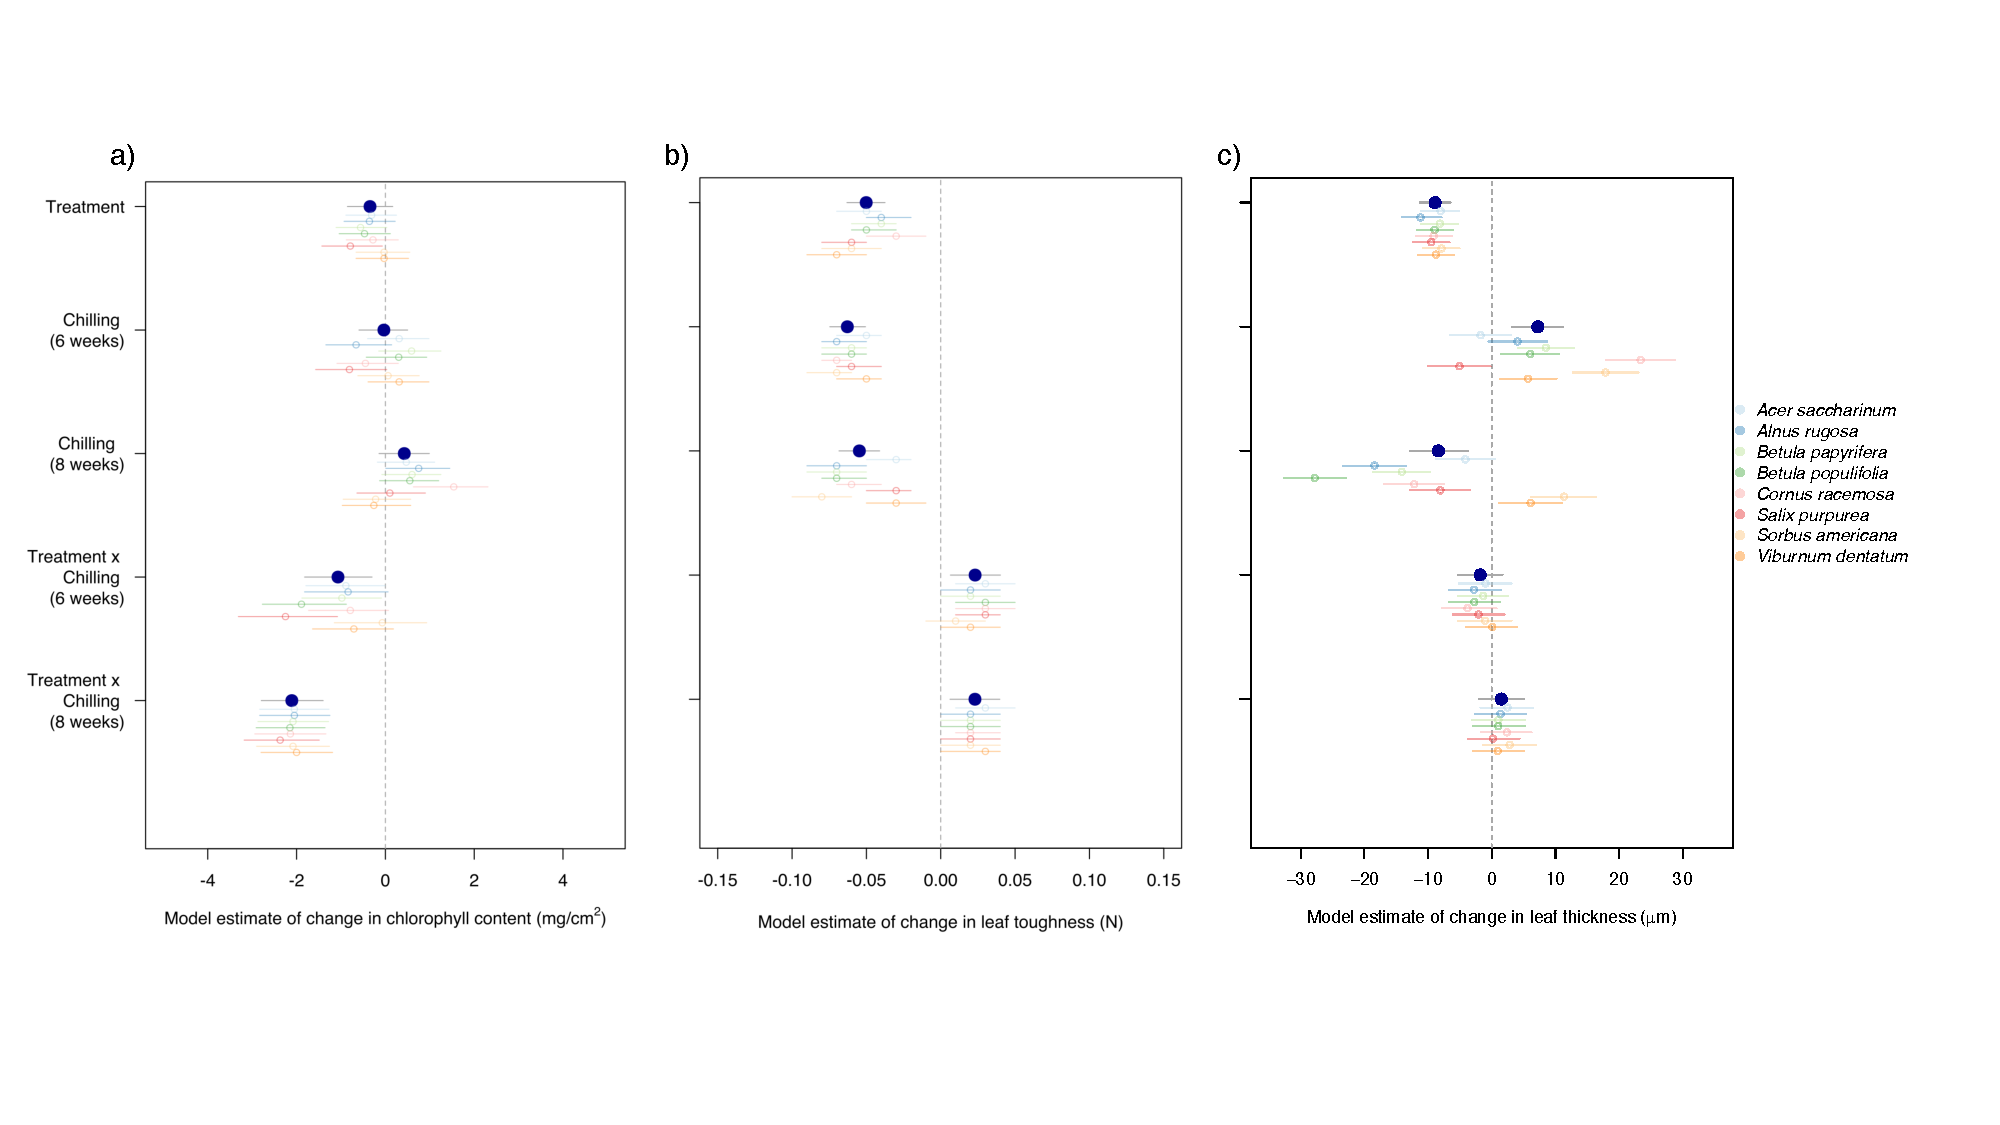
\includegraphics[width=18cm]{..//analyses/figures/mu_leaftraits.pdf} 
  -\caption{Effects of false spring treatment, six weeks of chilling and eight weeks of chilling on a) leaf toughness (N) and b) leaf thickness ($\mu$m). Dots and thin lines show means and 90\% uncertainty intervals and thicker lines show 50\% uncertainty intervals. }\label{fig:muleaf}
  -\end{center}
  -\end{figure}}
  
  {\begin{figure} [H]
  -\begin{center}
  -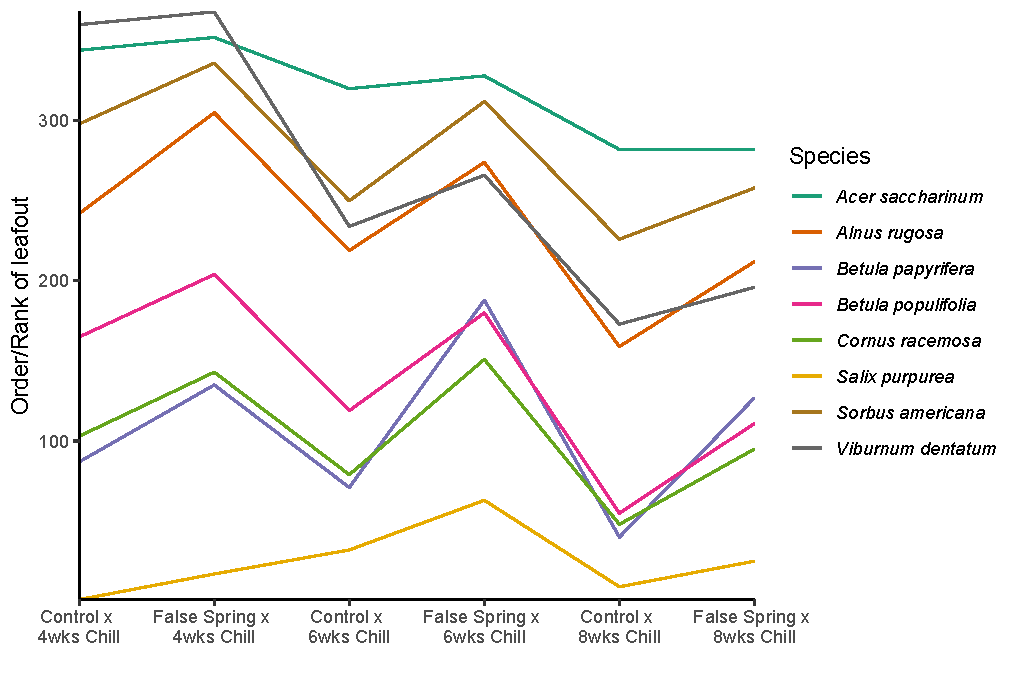
\includegraphics[width=12cm]{..//analyses/figures/leafoutorder_byrank.pdf} 
  -\caption{Understanding rank order of leafout across all species using (a) mean trends and (b) raw estimates. }\label{fig:rank}
  -\end{center}
  -\end{figure}}
  

\end{document}
